\documentclass {article}

\usepackage{amsmath}
\usepackage{graphics}
\usepackage{color}

\newcommand\conf{\mathbf{q}}

\title {Contact surface constraints}

\begin {document}
\maketitle

\section {Definition}

A contact constraint is defined by
\begin{itemize}
\item a set of convex planar polygons called \textit{object contact surfaces}
  $(o_i)_{i\in I}$,
\item a set of convex planar polygons called \textit{floor contact surfaces}
  $(f_i)_{i\in J}$.
\end{itemize}
We denote respectively by $\bar{I}$ and $\bar{J}$ the cardinal of $I$ and $J$.
To each contact surface, we associate a coordinate frame in such a way that
\begin{itemize}
\item the origin of the coordinate frame is the barycenter of the vertices,
\item the $x$ axis is normal to the polygon plane,
\end{itemize}
\section {Distance between floor and object contact surfaces}
\begin{figure}
  \centerline {
    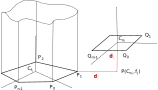
\includegraphics{figures/convex-shape-contact.pdf}
  }
  \caption{Distance between two convex contact surfaces.}
  \label{fig:distance}
\end{figure}

The distance $d(o_i, f_j)$ between object surface $o_i$ and
environment surface $ f_j $ is defined by:
\begin{equation*}
  d(o_i,f_j)^2 =
  \left\lbrace \begin{array}{cl}
    d_{\parallel}^2 + d_{\perp}^2 &, \text{ if } d_{\parallel} > 0 \\
    d_{\perp}^2                   &, \text{ otherwise}
  \end{array} \right.
\end{equation*}
where
\begin{itemize}
\item $P (C_{o_i}, f_j)$ is the projection of the center of $o_i$ onto the plane containing $ f_j $,
\item $\mathbf{n}_{f_j}$ is the normal of $ f_j $,
\item $d_{\parallel} = d(f_j, P (C_{o_i}, f_j))$ is the distance returned by \texttt{ConvexShapeData::distance},
\item $d_{\perp} = \mathbf{n}_{f_j}.\vec{C_{f_j} C_{o_i}}$ is the distance along the normal of $ f_j $,
\end{itemize}

\section{Numerical constraints achieving contact: current implementation}
\label{eq:current implementation}

We denote by $\conf$ the configuration of the robot. In the current
implementation of \texttt{ConvexShapeContact}, the value
$h_{contact}(\conf)$ of the constraint is of dimension 5 and computed
as follows.
\begin{itemize}
\item Let $i\in I$, $j\in J$ be the indices of the object and
  environment polygons that minimize $d (o_i, f_j)$.
\item Let $\mathbf{u} = (u_x,u_y,u_z,u_{rx},u_{ry},u_{rz}) = \log_{R^3\times SO(3)}(f_j^{-1} o_{i})$ represent the 6d pose
  error of $o_i$ frame with respect to $f_j$ frame.
\end{itemize}
\begin{enumerate}
  \item $h_{contact}(\conf) = (x+m,y,z,ry,rz)$ if $P(C_{o_i},f_j)$ is outside
    polygon $f_j$,
  \item $h_{contact}(\conf) = (x+m,0,0,ry,rz)$ if $P(C_{o_i},f_j)$ is inside polygon $f_j$,
\end{enumerate}
where $m$ is a margin used to avoid collision between the objects holding the
surfaces. It can also be used to define preplacement configurations.

\paragraph{Geometric interpretation.} When object $o_i$ is not "above" surface $f_j$ (case 1), the numerical resolution tries to bring the origin of $o_i$ to the origin of $f_j$. Once the object is above $f_j$, the translation in the plane of $f_j$ is not constrained anymore.

\paragraph{Problem~1.} The probability density of the position of the object on the surface when solving the constraint from a random configuration depends on the numerical resolution algorithm.

\subsection{Complement constraint}
With the same notation, the complement constraint is defined by
\begin{itemize}
  \item $h_{complement}(\conf) = (0,0,rx)$ if $P(C_{o_i},f_j)$ is outside polygon $f_j$,
  \item $h_{complement}(\conf) = (y,z,rx)$ if $P(C_{o_i},f_j)$ is inside polygon $f_j$,
\end{itemize}

\paragraph{Problem~2.}
In the current implementation, a given value for the right hand side
of the complement constraint may correspond to several distinct poses
of the object: potentially one per pair $(o_i, f_j)$. A bad
consequence is that keeping the complement constraint constant along a
path may produce a path where the object jumps from one contact to
another one.

\section{Numerical constraints achieving contact: new implementation}

We keep the same definition for the contact constraint.

\subsection{Complement constraint}

Let $M$ be an upper bound of the coordinates of all vertices of all $(f_j)_{j\in J}$:
$$
\forall j\in J,\ \mbox{for all vertices}\ P = (x,y) \ \mbox{of} \ f_j,
\ |x| \leq M, |y| \leq M
$$
Coordinates $(x,y)$ are expressed in the local frame of the polygon. Then, with
the same notation as previously,
\begin{itemize}
\item $h_{complement}(\conf) = (2j.M, 2i.M,rx)$ if $P(C_{o_i},f_j)$ is outside
  polygon $f_j$,
\item $h_{complement}(\conf) = (2j.M + y, 2i.M + z,rx)$ if $P(C_{o_i},f_j)$ is
  inside polygon $f_j$,
\end{itemize}

\paragraph{Property 1.} Function $h_{complement}$ above is injective over the
solution set of the contact constraint $h_{contact}(\conf)=0$.

Property 1 is due to the fact that $y$ and $z$ in the expression of $h_{complement}$ are always less than $M$ in absolute value.

\subsection {Combination of contact and complement constraints}

\paragraph{Hypothesis.} All the contact surfaces $(o_i)_{i\in I}$ are hold by a
same joint denoted by $J_{obj}$.

 If $J_{obj}$ is a freeflyer, the configuration variables of the
 freeflyer joint can be computed explicitely from
\begin{itemize}
\item the position of the contact surface $f_j$ that realizes the contact,
\item the right hand side of $h_{complement}$ denoted as $(Y,Z,RX)$.
\end{itemize}
The input configuration variables of this explicit constraints are the
configuration variables of the joints that move at least one $f_j$, for $j\in J$.

\paragraph{Computation of the output value.} We first determine which polygons
are in contact:
\begin{eqnarray*}
j &=& \lfloor \frac{Y}{2M} + \frac{1}{2} \rfloor\\
i &=& \lfloor \frac{Z}{2M} + \frac{1}{2} \rfloor
\end{eqnarray*}
we can then determine the right hand side of the \texttt{explicit\_::RelativePose} instance, denoted $RP_{i,j}$ that computes configuration of $J_{obj}$ as:
\begin{eqnarray*}
  y &=& Y - j.M \\
  x &=& Z - i.M \\
  rx &=& RX
\end{eqnarray*}

\paragraph{Implementation details.} We define a class deriving from
\texttt{Implicit}, named \texttt{explicit\_::ConvexShapeContact} and
that takes as input a \texttt{ConvexShapeContact} instance.

Note that to determine the input configuration variables, we need the \texttt{ConvexShapeContact} instance to be already initialized with all $(f_j)_{j\in J}$
polygons.

For each pair $(f_j, o_i)$, we create an instance of \texttt{explicit\_::RelativePose} with as inputs:
\begin{itemize}
  \item \texttt{joint1}: the joint that holds $f_j$,
  \item \texttt{joint2}: the joint that holds $o_i$,
  \item \texttt{frame1}: the position of $f_j$ in \texttt{joint1},
  \item \texttt{frame2}: the position of $o_i$ in \texttt{joint2},
  \item \texttt{mask}: \texttt{(true,true,true,true,true,true)},
  \item \texttt{comp}: \texttt{(EqualToZero,Equality,Equality,Equality,EqualToZero,EqualToZero)}.
\end{itemize}

The output function $f$ returns $I_{SE(3)}$ whatever the input is. The correct
value is computed through virtual method \texttt{implicitToExplicitRhs} that
will compute the position of $J_{obj}$ using $RP_{i,j}$. Let us recall that
$$
\conf_{obj} = f(\conf_{in}) + rhs = rhs
$$

\paragraph{Problem~3:} The Jacobian will alway be filled with 0. This will work
when the floor surface is hold by static parts of the environment only. This is
already the case with the current implementation that uses \texttt{LockedJoint}
class.
\end{document}






\section{Numerical constraints achieving contact: new implementation}

We propose to add a dimension to the contact constraint value to store
a discrete value that encodes which pair $(o_i, f_j)$ is in contact.

With the same notation as in Section~\ref{eq:current implementation},
\begin{enumerate}
  \item $h(\conf) = (x+m,y,z,ry,rz,\sigma)$ if $P(C_{o_i},f_j)$ is outside
    polygon $f_j$,
  \item $h(\conf) = (x+m,0,0,ry,rz,\sigma)$ if $P(C_{o_i},f_j)$ is
    inside polygon $f_j$,
\end{enumerate}
where $\sigma (\conf) = j.\bar{J} + i$.

\subsection{Complement constraint}

We add the same dimension to the constraint complement value as in the
previous section:
\begin{itemize}
\item $h(\conf) = (0,0,rx,\sigma)$ if $P(C_{o_i},f_j)$ is outside polygon
  $f_j$,
\item $h(\conf) = (y,z,rx,\sigma)$ if $P(C_{o_i},f_j)$ is inside polygon $f_j$,
\end{itemize}

\paragraph{Note~1:} functions $h$ defined above are not differentiable
functions. They are piecewise constant. However, this should not harm
the numerical resolution algorithm.
\paragraph{Note~2:} The combination of the contact constraint and its complement
can be implemented as a relative pose constraint between the joints supporting
$f_j$ and $o_j$. Moreover, if the joint supporting $o_j$ is a freeflyer, the
constraint is explicit.
